\scanpage{100}
\mspage{99}

\unsure{pris|prise} pour donner un sens intrinsèque aux ``supports constructibles'', via les $\deleted{\unsure{A}}\unsure{X^\circ|X^0|X^o}$,

\uline{26 juin} Il sera peut-être plus simple, \unsure{puisque} pratiquement je suis obligé ici \deleted{de} (pour \unsure{ma|la} façon de définir $X^\circ$ par un ``support'' au sens $\parallel$) \deleted{du fait} d'admettre Ax L1 (en plus de Ax L2, Ax L3), autant le définir plus simplement comme
\[
X^\circ=\operatorname{Supp}\operatorname{omb}(X)^\circ
\]
c'est pareil grâce au cor. p.86 et au fait que \deleted{les $Y\in\unsure{\operatorname{Ouv}|\operatorname{Om}}$ \unsure{pour tout}} par Ax L2, pour toute partie support $\deleted{\unsure{B}}S$ de $M$, on a
\[
S=\operatorname{supp}(S\cap\unsure{\mathcal L|L}).
\]
(plus gén\textsuperscript{t}, si $S$ est fermé pour $\ll$, on a
\[
\operatorname{supp}S=\operatorname{Supp}(S\cap\mathcal L)\text{)}.
\]

Notons \unsure{\(\dagger\)|t} (pour nous rassurer)

\uline{Lemme} Soit $\deleted{\unsure{X}}F\unsure{\preccurlyeq|\prec|\leq}X$, \deleted{et} et considérons
\margin{$\big\vert\!\big\vert$}
\[
\unsure{\varphi|\phi}:\widetilde F\longrightarrow\widetilde X,\quad\text{soit}\quad\widetilde F^\circ=\varphi^{-1}(\{X\})=\{X'\in\widetilde F\mid \overbrace{X'^\circ\ll X}^{\inserted{\text{i.e. }X'^\circ\subset X^\circ}}\}.
\]
Alors
\[
\begin{aligned}
X^\circ&=\underset{X'\in\widetilde F^\circ}{\operatorname{Sup}}_\Sigma X'^\circ
\left(=\operatorname{Supp}\bigcup_{X'\in\widetilde F^\circ}X'^\circ\quad\deleted{=\operatorname{Supp}\bigcup}\right.\\
&\hspace{5em}\left.=\operatorname{Supp}\bigcup_{X'\in\unsure{\widetilde F|\widetilde F^\circ}}\operatorname{omb}(X')^\circ\right)
\end{aligned}
\]
Pourtant, dans le \unsure{cas quasi-ensembliste}, on \unsure{n'aura} en général pas
\[
\operatorname{omb}_{\ll}(X)^\circ=\bigcup_{X'\in\widetilde F^\circ}\operatorname{omb}(X')^\circ.
\]
\margin{\figure{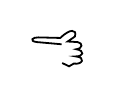
\begin{tikzpicture}[scale=.35]
\draw[line width=.65pt] (0,0) -- (-.9,.08) .. controls (-1.2,.12) and (-1.05,.26) .. (-.85,.25) -- (-.05,.23) .. controls (.3,.57) and (.57,.56) .. (.48,.28) -- (.22,.1) -- (.58,.08) .. controls (.78,.04) and (.77,-.15) .. (.53,-.18) .. controls (.86,-.23) and (.79,-.45) .. (.51,-.44) .. controls (.88,-.47) and (.77,-.75) .. (.44,-.7) -- (.27,-.8) -- (.02,-.68);
\end{tikzpicture}}}
L'inclusion $\supset$ est évidente du fait que les $X'^\circ$ sont $\subset X^\circ$. Prouvons $\subset$.
\deleted{Donc} Cela équivaut au
